\section{Рабочий проект}

\subsection{Спецификация компонентов программной системы}

В данном подразделе приводится описание основных компонентов разработанной программной системы. Рабочий проект отражает не проектные решения базы данных и архитектуры, рассмотренные ранее, а фактический состав программных компонентов, реализующих функции web-платформы для поиска работы и подбора IT-специалистов.

Разработанная система построена как клиент-серверное web-приложение. Серверная часть обеспечивает обработку запросов, выполнение бизнес-логики, аутентификацию пользователей, разграничение прав доступа и взаимодействие с базой данных. Клиентская часть предоставляет пользователям web-интерфейс для работы с вакансиями, профилями, компаниями, откликами, избранными вакансиями и административными функциями.

Компоненты программной системы сгруппированы по функциональным областям: аутентификация и авторизация, работа с профилем соискателя, управление компаниями работодателей, обработка вакансий, откликов, избранных вакансий и навыков, а также выполнение административных действий. Отдельно рассматривается клиентская часть, обеспечивающая взаимодействие пользователя с системой через страницы web-интерфейса и запросы к серверному приложению.

Модели данных не выделяются в отдельный подраздел рабочего проекта, так как проект базы данных был подробно рассмотрен в разделе 3.5. В данном разделе модели упоминаются в составе тех компонентов, в которых они используются.

\subsubsection{Компоненты аутентификации и авторизации}

Компоненты аутентификации и авторизации обеспечивают регистрацию пользователей, вход в систему, завершение сеанса, получение сведений о текущем пользователе и разграничение доступа к функциям программной системы. Данная подсистема является базовой для работы остальных компонентов, так как большинство операций платформы зависит от роли пользователя и факта его авторизации.

В системе предусмотрена регистрация пользователей с ролями соискателя и работодателя. При регистрации пользователь указывает адрес электронной почты, пароль, имя и роль. Серверная часть выполняет проверку заполнения обязательных полей, проверяет допустимость выбранной роли, контролирует уникальность адреса электронной почты и сохраняет пароль в базе данных в виде хэша. Такой подход исключает хранение паролей в открытом виде.

Вход в систему выполняется по адресу электронной почты и паролю. После успешной проверки учётных данных сервер формирует JWT-токен, содержащий идентификатор пользователя, адрес электронной почты и роль. Сформированный токен сохраняется в cookie, после чего используется при обращении к защищённым маршрутам приложения.

Проверка авторизованного пользователя выполняется промежуточным обработчиком, который извлекает токен из cookie, проверяет его корректность и загружает сведения о пользователе из базы данных. Если токен отсутствует, недействителен или пользователь заблокирован, выполнение защищённого запроса прекращается с соответствующим сообщением об ошибке. Разграничение доступа по ролям реализовано отдельным middleware, который проверяет, входит ли роль текущего пользователя в список ролей, которым разрешено выполнение конкретного действия.

Основные компоненты подсистемы аутентификации и авторизации представлены в таблице \ref{auth:table}.

\renewcommand{\arraystretch}{0.9}
\begin{xltabular}{\textwidth}{|p{4.2cm}|p{4.1cm}|X|}
	\caption{Компоненты аутентификации и авторизации}
	\label{auth:table}\\
	\hline
	Компонент & Файл & Назначение \\
	\hline
	\endfirsthead
	
	\caption*{Продолжение таблицы \ref{auth:table}}\\
	\hline
	Компонент & Файл & Назначение \\
	\hline
	\finishhead
	
	Маршруты аутентификации & \texttt{auth.routes.js} & Определяют API-маршруты регистрации, входа, получения текущего пользователя и выхода из системы. \\
	\hline
	Контроллер аутентификации & \texttt{auth.controller.js} & Обрабатывает HTTP-запросы, вызывает сервисные функции регистрации и входа, формирует ответ клиентской части, устанавливает и очищает cookie с JWT-токеном. \\
	\hline
	Сервис аутентификации & \texttt{auth.service.js} & Реализует основную логику регистрации и входа: проверку входных данных, проверку уникальности электронной почты, хэширование пароля, проверку пароля и признака блокировки пользователя. \\
	\hline
	Генератор токена & \texttt{generate-token.js} & Формирует JWT-токен на основе идентификатора пользователя, электронной почты и роли пользователя. \\
	\hline
	Middleware авторизации & \texttt{auth.middleware.js} & Проверяет наличие и корректность JWT-токена, получает данные пользователя из базы данных и добавляет их в объект запроса для дальнейшей обработки. \\
	\hline
	Middleware проверки ролей & \texttt{role.middleware.js} & Ограничивает доступ к маршрутам в зависимости от роли пользователя и предотвращает выполнение действий, не предусмотренных для соответствующей роли. \\
	\hline
	Модель пользователя & \texttt{user.js} & Хранит учётные данные пользователя, его роль, ФИО и признак блокировки, а также связывает пользователя с профилем соискателя, компанией и избранными вакансиями. \\
	\hline
\end{xltabular}
\renewcommand{\arraystretch}{1.0}

Таким образом, подсистема аутентификации и авторизации обеспечивает защищённый доступ к функциям web-платформы, связывает пользователя с его ролью и создаёт основу для разграничения возможностей соискателя, работодателя и администратора.


\subsubsection{Компоненты работы с профилем соискателя}

Компоненты работы с профилем соискателя обеспечивают создание, просмотр и редактирование профессиональной информации пользователя с ролью соискателя. Профиль используется для хранения сведений о специализации, описания опыта и ссылки на GitHub-профиль, а также для связи соискателя с набором профессиональных навыков и откликами на вакансии.

Создание профиля доступно только авторизованному пользователю с ролью соискателя. При создании профиля серверная часть проверяет наличие обязательного поля специализации, корректность переданных текстовых данных и отсутствие уже созданного профиля у текущего пользователя. Это ограничение необходимо для того, чтобы одному пользователю соответствовал только один профиль соискателя.

Редактирование профиля также выполняется только владельцем профиля. Перед изменением данных сервер проверяет существование профиля и принадлежность профиля текущему пользователю. Пользователь может изменить специализацию, описание и ссылку на GitHub. Если запрос не содержит данных для изменения, сервер возвращает сообщение об ошибке.

Отдельной частью компонента является управление навыками соискателя. При добавлении навыка выполняется проверка названия навыка, поиск уже существующего навыка в базе данных и создание нового навыка при его отсутствии. Связь между профилем и навыком сохраняется через промежуточную таблицу. Если указанный навык уже добавлен в профиль, повторное добавление не выполняется. Удаление навыка из профиля также доступно только владельцу профиля.

Для работодателя реализован просмотр профилей соискателей. Работодатель может получить список профилей, а также просмотреть конкретный профиль по идентификатору. При получении списка поддерживается фильтрация по специализации и навыку, что позволяет использовать профиль соискателя не только как личную карточку пользователя, но и как источник данных для поиска кандидатов.

Основные компоненты работы с профилем соискателя представлены в таблице \ref{candidateProfile:table}.

\renewcommand{\arraystretch}{0.9}
\begin{xltabular}{\textwidth}{|p{4.0cm}|p{4.9cm}|>{\raggedright\arraybackslash}X|}
	\caption{Компоненты работы с профилем соискателя\label{candidateProfile:table}}\\
	\hline
	Компонент & Файл & Назначение \\
	\hline
	\endfirsthead
	
	\caption*{Продолжение таблицы \ref{candidateProfile:table}}\\
	\hline
	Компонент & Файл & Назначение \\
	\hline
	\endhead
	
	Маршруты профиля соискателя & \texttt{candidate-profile.}\newline\texttt{routes.js} & Определяют API-маршруты создания, получения и редактирования профиля соискателя, управления навыками, а также просмотра профилей соискателей работодателем. \\
	\hline
	Контроллер профиля соискателя & \texttt{candidate-profile.}\newline\texttt{controller.js} & Обрабатывает запросы, связанные с профилем соискателя: создание профиля, получение собственного профиля, обновление данных, добавление и удаление навыков, получение списка профилей и просмотр профиля по идентификатору. \\
	\hline
	Модель профиля соискателя & \texttt{candidateProfile.js} & Хранит сведения о специализации, описании и ссылке на GitHub, связывает профиль с пользователем, навыками и откликами на вакансии. \\
	\hline
	Модель навыка & \texttt{skill.js} & Хранит справочник навыков, которые могут быть связаны с профилями соискателей и вакансиями. \\
	\hline
	Связующая модель навыков соискателя & \texttt{candidateSkill.js} & Реализует связь между профилем соискателя и навыком, позволяя одному профилю иметь несколько навыков. \\
	\hline
	Модель пользователя & \texttt{user.js} & Используется для связи профиля соискателя с учётной записью пользователя и отображения основных сведений о пользователе при просмотре профиля работодателем. \\
	\hline
\end{xltabular}
\renewcommand{\arraystretch}{1.0}

Таким образом, компоненты работы с профилем соискателя обеспечивают хранение профессиональной информации пользователя, управление навыками и предоставляют работодателю возможность поиска кандидатов по специализации и набору навыков.

\subsubsection{Компоненты работы с компаниями работодателей}

Компоненты работы с компаниями работодателей обеспечивают создание, просмотр и редактирование профиля компании, от имени которой работодатель публикует вакансии. Данный компонент связывает учётную запись работодателя с информацией об организации и используется в дальнейшем при создании и отображении вакансий.

Создание компании доступно только авторизованному пользователю с ролью работодателя. При создании профиля компании серверная часть проверяет наличие обязательного поля названия компании, а также корректность переданных текстовых данных. Для одного работодателя допускается создание только одной компании, поэтому перед сохранением новой записи выполняется проверка существования компании, связанной с текущим пользователем.

Получение сведений о компании выполняется двумя способами. Работодатель может получить данные собственной компании, связанные с его учётной записью. Также предусмотрено получение компании по идентификатору, что используется при просмотре сведений о работодателе и связанных с ним вакансиях. При обращении к несуществующей компании сервер возвращает сообщение об ошибке.

Редактирование компании выполняется только владельцем соответствующего профиля. Перед изменением данных серверная часть получает компанию текущего работодателя и проверяет, совпадает ли её идентификатор с идентификатором, указанным в запросе. Если пользователь пытается изменить чужую компанию, выполнение операции запрещается. Работодатель может изменить название компании, описание и адрес сайта.

Модель компании связана с моделью пользователя и моделью вакансии. Связь с пользователем позволяет определить владельца компании, а связь с вакансиями позволяет отображать список вакансий, опубликованных конкретным работодателем.

Основные компоненты работы с компаниями работодателей представлены в таблице \ref{company:table}.

\renewcommand{\arraystretch}{0.9}
\begin{xltabular}{\textwidth}{|p{4.4cm}|p{4.2cm}|X|}
	\caption{Компоненты работы с компаниями работодателей\label{company:table}}\\
	\hline
	Компонент & Файл & Назначение \\
	\hline
	\endfirsthead
	
	\caption*{Продолжение таблицы \ref{company:table}}\\
	\hline
	Компонент & Файл & Назначение \\
	\hline
	\endhead
	
	Маршруты компаний & \texttt{company.routes.js} & Определяют API-маршруты получения собственной компании, создания компании, редактирования компании и получения компании по идентификатору. \\
	\hline
	Контроллер компаний & \texttt{company.controller.js} & Обрабатывает запросы, связанные с компаниями работодателей: получение компании текущего пользователя, создание нового профиля компании, обновление данных компании и получение компании по идентификатору. \\
	\hline
	Модель компании & \texttt{company.js} & Хранит название компании, описание и адрес сайта, связывает компанию с учётной записью работодателя и опубликованными вакансиями. \\
	\hline
	Модель пользователя & \texttt{user.js} & Используется для определения работодателя, которому принадлежит компания. \\
	\hline
	Модель вакансии & \texttt{vacancy.js} & Используется для связи компании с вакансиями, которые публикуются работодателем от имени данной компании. \\
	\hline
	Middleware авторизации & \texttt{auth.middleware.js} & Проверяет, что пользователь авторизован перед выполнением операций с компанией. \\
	\hline
	Middleware проверки ролей & \texttt{role.middleware.js} & Ограничивает доступ к операциям с компаниями только для пользователей с ролью работодателя. \\
	\hline
\end{xltabular}
\renewcommand{\arraystretch}{1.0}

Таким образом, компоненты работы с компаниями работодателей обеспечивают хранение сведений об организации, связывают работодателя с публикуемыми вакансиями и предотвращают изменение данных компании пользователями, не являющимися её владельцами.

\subsubsection{Компоненты работы с вакансиями}

Компоненты работы с вакансиями обеспечивают создание, просмотр, редактирование, публикацию и снятие с публикации предложений о работе. Вакансия является одной из центральных сущностей программной системы, так как через неё осуществляется взаимодействие между работодателем и соискателем.

Создание вакансии доступно авторизованному пользователю с ролью работодателя. Перед созданием вакансии серверная часть проверяет наличие у работодателя профиля компании, так как каждая вакансия должна быть связана с конкретной организацией. При обработке запроса проверяется заполнение обязательных полей: названия вакансии, специализации, описания, требований, типа занятости и формата работы. Также выполняется проверка допустимости значений перечислимых полей, таких как тип занятости и формат работы.

После создания вакансия сохраняется со статусом черновика. Такой подход позволяет работодателю сначала подготовить описание вакансии, а затем отдельно опубликовать её. Опубликованные вакансии доступны для просмотра всем пользователям, включая неавторизованных посетителей. При получении списка опубликованных вакансий поддерживается поиск и фильтрация по ключевым параметрам, включая поисковую строку, специализацию, формат работы, тип занятости и навык.

Редактирование вакансии доступно только работодателю, которому принадлежит компания, разместившая данную вакансию. Перед изменением данных серверная часть проверяет существование компании текущего пользователя, наличие указанной вакансии и её принадлежность данной компании. Если пользователь пытается изменить чужую вакансию, операция не выполняется. При редактировании допускается изменение текстовых данных, сведений о зарплате и местоположении, а также типа занятости и формата работы.

Публикация вакансии переводит её в статус опубликованной, после чего она становится доступной в общем списке вакансий. Снятие с публикации переводит вакансию в архивный статус. Для работодателя такая операция используется для управления собственными вакансиями, а для администратора — в рамках модерации содержимого платформы.

Отдельной частью компонента является управление навыками вакансии. Работодатель может добавить к вакансии требуемый навык или удалить ранее добавленный навык. При добавлении навыка сервер проверяет наличие названия навыка, ищет существующую запись в справочнике навыков и создаёт новую запись при её отсутствии. Повторное добавление одного и того же навыка к вакансии не допускается.

Основные компоненты работы с вакансиями представлены в таблице \ref{vacancy:table}.

\renewcommand{\arraystretch}{0.9}
\begin{xltabular}{\textwidth}{|p{4.4cm}|p{4.2cm}|X|}
	\caption{Компоненты работы с вакансиями\label{vacancy:table}}\\
	\hline
	Компонент & Файл & Назначение \\
	\hline
	\endfirsthead
	
	\caption*{Продолжение таблицы \ref{vacancy:table}}\\
	\hline
	Компонент & Файл & Назначение \\
	\hline
	\endhead
	
	Маршруты вакансий & \texttt{vacancy.routes.js} & Определяют API-маршруты создания вакансии, получения опубликованных вакансий, просмотра вакансии по идентификатору, получения вакансий текущего работодателя, редактирования, публикации, снятия с публикации и управления навыками вакансии. \\
	\hline
	Контроллер вакансий & \texttt{vacancy.controller.js} & Обрабатывает HTTP-запросы, связанные с вакансиями, вызывает сервисные функции и формирует ответы клиентской части. \\
	\hline
	Сервис вакансий & \texttt{vacancy.service.js} & Реализует основную бизнес-логику работы с вакансиями: проверку компании работодателя, валидацию обязательных полей, фильтрацию опубликованных вакансий, изменение статуса вакансии и управление навыками. \\
	\hline
	Модель вакансии & \texttt{vacancy.js} & Хранит сведения о вакансии, включая название, специализацию, описание, требования, зарплату, местоположение, тип занятости, формат работы, статус публикации и связь с компанией. \\
	\hline
	Модель компании & \texttt{company.js} & Используется для проверки принадлежности вакансии работодателю и связи вакансии с организацией, разместившей предложение о работе. \\
	\hline
	Модель навыка & \texttt{skill.js} & Используется для хранения справочника навыков, которые могут быть добавлены к вакансии как требования к кандидату. \\
	\hline
	Связующая модель навыков вакансии & \texttt{vacancySkill.js} & Реализует связь между вакансией и навыком, позволяя одной вакансии содержать несколько требуемых навыков. \\
	\hline
	Middleware авторизации & \texttt{auth.middleware.js} & Проверяет авторизацию пользователя перед выполнением операций работодателя с вакансиями. \\
	\hline
	Middleware проверки ролей & \texttt{role.middleware.js} & Ограничивает создание, редактирование, публикацию и снятие вакансий с публикации в зависимости от роли пользователя. \\
	\hline
\end{xltabular}
\renewcommand{\arraystretch}{1.0}

Таким образом, компоненты работы с вакансиями обеспечивают полный жизненный цикл вакансии: от создания черновика работодателем до публикации, поиска соискателями, редактирования, архивирования и связывания с требуемыми профессиональными навыками.

\subsubsection{Компоненты работы с откликами}

Компоненты работы с откликами обеспечивают взаимодействие между соискателем и работодателем после публикации вакансии. Отклик используется для фиксации заинтересованности соискателя в конкретной вакансии и позволяет работодателю рассматривать поступившие заявки от кандидатов.

Создание отклика доступно только авторизованному пользователю с ролью соискателя. Перед созданием отклика серверная часть проверяет наличие профиля соискателя, так как отклик должен быть связан не только с учётной записью пользователя, но и с его профессиональным профилем. Также проверяется существование вакансии и её статус. Отклик может быть создан только на опубликованную вакансию.

Для предотвращения дублирования заявок серверная часть проверяет, не был ли уже создан отклик текущего соискателя на выбранную вакансию. Если отклик уже существует, повторное создание не выполняется, а клиентской части возвращается сообщение об ошибке. При успешном создании отклик получает начальный статус \texttt{new}.

Соискатель может просматривать список собственных откликов. При получении списка откликов сервер возвращает данные о вакансиях, на которые пользователь отправлял заявки, а также сведения о компаниях, разместивших эти вакансии. Это позволяет соискателю отслеживать историю своих обращений и текущий статус каждого отклика.

Работодатель может просматривать отклики, поступившие на принадлежащие ему вакансии. Перед выдачей списка откликов серверная часть проверяет наличие компании у текущего работодателя и принадлежность указанной вакансии данной компании. В ответе возвращаются сведения о профиле соискателя, пользователе и навыках кандидата.

Изменение статуса отклика доступно только работодателю, которому принадлежит вакансия. Для отклика предусмотрены статусы \texttt{new}, \texttt{in\_review}, \texttt{accepted} и \texttt{rejected}. При изменении статуса сервер проверяет допустимость нового значения, существование отклика и принадлежность связанной вакансии компании текущего работодателя.

Основные компоненты работы с откликами представлены в таблице \ref{application:table}.

\renewcommand{\arraystretch}{0.9}
\begin{xltabular}{\textwidth}{|p{4.4cm}|p{4.2cm}|X|}
	\caption{Компоненты работы с откликами\label{application:table}}\\
	\hline
	Компонент & Файл & Назначение \\
	\hline
	\endfirsthead
	
	\caption*{Продолжение таблицы \ref{application:table}}\\
	\hline
	Компонент & Файл & Назначение \\
	\hline
	\endhead
	
	Маршруты откликов & \texttt{application.routes.js} & Определяют API-маршруты создания отклика, получения собственных откликов соискателя и изменения статуса отклика работодателем. \\
	\hline
	Маршрут просмотра откликов на вакансию & \texttt{vacancy.routes.js} & Связывает просмотр откликов с конкретной вакансией работодателя и передаёт обработку в контроллер откликов. \\
	\hline
	Контроллер откликов & \texttt{application.controller.js} & Обрабатывает HTTP-запросы, связанные с откликами: создание отклика, получение откликов соискателя, получение откликов на вакансию работодателя и изменение статуса отклика. \\
	\hline
	Сервис откликов & \texttt{application.service.js} & Реализует бизнес-логику работы с откликами: проверку профиля соискателя, проверку опубликованной вакансии, запрет повторного отклика, получение списков откликов и изменение статуса. \\
	\hline
	Модель отклика & \texttt{application.js} & Хранит связь между вакансией и профилем соискателя, статус отклика и дату его создания. \\
	\hline
	Модель профиля соискателя & \texttt{candidateProfile.js} & Используется для связи отклика с профессиональным профилем пользователя и отображения данных кандидата работодателю. \\
	\hline
	Модель вакансии & \texttt{vacancy.js} & Используется для связи отклика с вакансией и проверки принадлежности вакансии компании работодателя. \\
	\hline
	Модель компании & \texttt{company.js} & Используется при проверке прав работодателя на просмотр и изменение откликов по принадлежащим ему вакансиям. \\
	\hline
	Middleware авторизации & \texttt{auth.middleware.js} & Проверяет авторизацию пользователя перед созданием, просмотром и изменением откликов. \\
	\hline
	Middleware проверки ролей & \texttt{role.middleware.js} & Ограничивает создание отклика ролью соискателя, а изменение статуса и просмотр откликов на вакансию ролью работодателя. \\
	\hline
\end{xltabular}
\renewcommand{\arraystretch}{1.0}

Таким образом, компоненты работы с откликами обеспечивают основной сценарий взаимодействия соискателя и работодателя: отправку заявки на опубликованную вакансию, просмотр истории откликов соискателем, рассмотрение кандидатов работодателем и изменение статуса отклика.

\subsubsection{Компоненты работы с избранными вакансиями}

Компоненты работы с избранными вакансиями обеспечивают сохранение интересующих соискателя предложений о работе в отдельном списке. Данный функционал позволяет пользователю с ролью соискателя вернуться к выбранным вакансиям позже и не выполнять повторный поиск среди общего списка опубликованных предложений.

Добавление вакансии в избранное доступно только авторизованному пользователю с ролью соискателя. Перед выполнением операции серверная часть проверяет корректность идентификатора вакансии, существование вакансии и её статус. В избранное может быть добавлена только опубликованная вакансия, доступная для просмотра пользователями платформы.

Для предотвращения дублирования записей серверная часть проверяет, не была ли выбранная вакансия уже добавлена в избранное текущим пользователем. Если связь между пользователем и вакансией уже существует, повторное добавление не выполняется, а клиентской части возвращается сообщение об ошибке.

Получение списка избранных вакансий выполняется по идентификатору текущего пользователя. При формировании ответа сервер возвращает не только записи избранного, но и связанные с ними сведения о вакансиях и компаниях. Это позволяет клиентской части отобразить пользователю полноценный список сохранённых предложений о работе.

Удаление вакансии из избранного также выполняется только текущим соискателем. Перед удалением сервер проверяет наличие соответствующей записи в избранном. Если вакансия не найдена в списке избранного пользователя, операция не выполняется и возвращается сообщение об ошибке.

Основные компоненты работы с избранными вакансиями представлены в таблице \ref{favorite:table}.

\renewcommand{\arraystretch}{0.9}
\begin{xltabular}{\textwidth}{|p{4.4cm}|p{4.2cm}|X|}
	\caption{Компоненты работы с избранными вакансиями\label{favorite:table}}\\
	\hline
	Компонент & Файл & Назначение \\
	\hline
	\endfirsthead
	
	\caption*{Продолжение таблицы \ref{favorite:table}}\\
	\hline
	Компонент & Файл & Назначение \\
	\hline
	\endhead
	
	Маршруты избранных вакансий & \texttt{favorite.routes.js} & Определяют API-маршруты получения списка избранных вакансий, добавления вакансии в избранное и удаления вакансии из избранного. \\
	\hline
	Контроллер избранных вакансий & \texttt{favorite.controller.js} & Обрабатывает HTTP-запросы, связанные с избранными вакансиями, проверяет корректность идентификатора вакансии и вызывает сервисные функции. \\
	\hline
	Сервис избранных вакансий & \texttt{favorite.service.js} & Реализует бизнес-логику работы с избранным: проверку опубликованной вакансии, запрет повторного добавления, получение списка избранных вакансий и удаление записи из избранного. \\
	\hline
	Модель избранной вакансии & \texttt{favoriteVacancy.js} & Хранит связь между пользователем и вакансией, добавленной в избранное. \\
	\hline
	Модель вакансии & \texttt{vacancy.js} & Используется для проверки существования и статуса вакансии, а также для отображения сведений о сохранённой вакансии. \\
	\hline
	Модель компании & \texttt{company.js} & Используется для отображения сведений о компании, разместившей вакансию, при получении списка избранных вакансий. \\
	\hline
	Middleware авторизации & \texttt{auth.middleware.js} & Проверяет авторизацию пользователя перед выполнением операций с избранными вакансиями. \\
	\hline
	Middleware проверки ролей & \texttt{role.middleware.js} & Ограничивает доступ к операциям с избранными вакансиями только для пользователей с ролью соискателя. \\
	\hline
\end{xltabular}
\renewcommand{\arraystretch}{1.0}

Таким образом, компоненты работы с избранными вакансиями позволяют соискателю сохранять интересующие предложения о работе, просматривать их в отдельном списке и удалять из избранного неактуальные вакансии.

\subsubsection{Компоненты работы с навыками}

Компоненты работы с навыками обеспечивают хранение и использование справочника профессиональных навыков в программной системе. Навыки применяются для описания компетенций соискателей и требований работодателей к кандидатам, поэтому данный компонент связан как с профилями соискателей, так и с вакансиями.

В системе используется единый справочник навыков. Каждая запись справочника содержит уникальное название навыка. Такой подход позволяет избежать дублирования одинаковых навыков и использовать одни и те же значения при заполнении профилей соискателей и описании требований к вакансиям.

Получение списка навыков выполняется через отдельный API-маршрут. Данный маршрут доступен авторизованным пользователям. При обращении к нему серверная часть возвращает список навыков, отсортированный по названию. Такой список может использоваться клиентской частью при выборе навыков для профиля соискателя или вакансии.

Связь навыков с профилями соискателей реализуется через промежуточную модель. Благодаря этому один профиль может иметь несколько навыков, а один и тот же навык может быть указан у разных соискателей. Аналогичным образом навыки связываются с вакансиями: одна вакансия может содержать несколько требуемых навыков, а один навык может использоваться в разных вакансиях.

Навыки также используются при поиске и фильтрации данных. Работодатель может отбирать кандидатов по требуемым навыкам, а соискатель может использовать навыки при поиске подходящих вакансий. Таким образом, компонент работы с навыками выполняет не только справочную, но и связующую функцию между основными сущностями системы.

Основные компоненты работы с навыками представлены в таблице \ref{skill:table}.

\renewcommand{\arraystretch}{0.9}
\begin{xltabular}{\textwidth}{|p{4.4cm}|p{4.2cm}|>{\raggedright\arraybackslash}X|}
	\caption{Компоненты работы с навыками\label{skill:table}}\tabularnewline
	\hline
	Компонент & Файл & Назначение \tabularnewline
	\hline
	\endfirsthead
	
	\caption*{Продолжение таблицы \ref{skill:table}}\tabularnewline
	\hline
	Компонент & Файл & Назначение \tabularnewline
	\hline
	\endhead
	
	Маршруты навыков & \texttt{skill.routes.js} & Определяют API-маршрут получения списка навыков, доступный авторизованным пользователям системы. \tabularnewline
	\hline
	Контроллер навыков & \texttt{skill.controller.js} & Обрабатывает HTTP-запрос на получение списка навыков и формирует ответ клиентской части. \tabularnewline
	\hline
	Сервис навыков & \texttt{skill.service.js} & Получает список навыков из базы данных и сортирует их по названию. \tabularnewline
	\hline
	Модель навыка & \texttt{skill.js} & Хранит уникальные названия навыков и связывает навыки с профилями соискателей и вакансиями. \tabularnewline
	\hline
	Связующая модель навыков соискателя & \texttt{candidateSkill.js} & Реализует связь между профилем соискателя и навыком. \tabularnewline
	\hline
	Связующая модель навыков вакансии & \texttt{vacancySkill.js} & Реализует связь между вакансией и требуемым навыком. \tabularnewline
	\hline
	Модель профиля соискателя & \texttt{candidateProfile.js} & Используется при привязке навыков к профессиональному профилю соискателя. \tabularnewline
	\hline
	Модель вакансии & \texttt{vacancy.js} & Используется при привязке навыков к требованиям конкретной вакансии. \tabularnewline
	\hline
	Middleware авторизации & \texttt{auth.middleware.js} & Проверяет авторизацию пользователя перед получением списка навыков. \tabularnewline
	\hline
\end{xltabular}
\renewcommand{\arraystretch}{1.0}


Таким образом, компоненты работы с навыками обеспечивают единое хранение профессиональных компетенций, связывают профили соискателей с требованиями вакансий и используются при поиске и фильтрации данных в системе.

\subsubsection{Административные компоненты программной системы}

Административные компоненты программной системы предназначены для выполнения действий по контролю пользователей и вакансий. Данный функционал доступен только пользователю с ролью администратора и используется для просмотра данных системы, ограничения доступа нарушающих правила пользователей и удаления некорректных или неактуальных вакансий.

Доступ к административным маршрутам защищён механизмами аутентификации и проверки роли пользователя. Перед выполнением административного действия серверная часть проверяет, что пользователь авторизован и обладает ролью администратора. Это предотвращает доступ обычных соискателей и работодателей к функциям управления системой.

Администратор может получить список пользователей, зарегистрированных в системе. При формировании ответа возвращаются основные сведения об учётных записях: идентификатор, адрес электронной почты, ФИО, роль и признак блокировки. Эти данные позволяют администратору контролировать состав пользователей и при необходимости ограничивать доступ отдельных учётных записей.

Блокировка пользователя выполняется по идентификатору. Перед выполнением операции сервер проверяет корректность переданного идентификатора и существование пользователя. Также предусмотрена дополнительная проверка, запрещающая администратору заблокировать собственную учётную запись. После успешного выполнения операции у пользователя устанавливается признак блокировки.

Администратор также может получить список вакансий, размещённых в системе. При получении списка вакансий дополнительно загружаются сведения о компании, которой принадлежит вакансия. Это позволяет администратору просматривать не только само предложение о работе, но и организацию, от имени которой оно было опубликовано.

Удаление вакансии выполняется по идентификатору. Перед удалением серверная часть проверяет корректность параметра маршрута и существование указанной вакансии. Если вакансия найдена, она удаляется из базы данных. Если вакансия отсутствует, клиентской части возвращается сообщение об ошибке.

Основные административные компоненты программной системы представлены в таблице \ref{admin:table}.

\renewcommand{\arraystretch}{0.9}
\begin{xltabular}{\textwidth}{|p{4.4cm}|p{4.2cm}|X|}
	\caption{Административные компоненты программной системы\label{admin:table}}\\
	\hline
	Компонент & Файл & Назначение \\
	\hline
	\endfirsthead
	
	\caption*{Продолжение таблицы \ref{admin:table}}\\
	\hline
	Компонент & Файл & Назначение \\
	\hline
	\endhead
	
	Административные маршруты & \texttt{admin.routes.js} & Определяют API-маршруты получения списка пользователей, получения списка вакансий, блокировки пользователя и удаления вакансии. \\
	\hline
	Административный контроллер & \texttt{admin.controller.js} & Обрабатывает HTTP-запросы администратора, проверяет корректность идентификаторов в параметрах маршрутов и вызывает сервисные функции. \\
	\hline
	Административный сервис & \texttt{admin.service.js} & Реализует бизнес-логику административных действий: получение пользователей, получение вакансий, блокировку пользователя и удаление вакансии. \\
	\hline
	Модель пользователя & \texttt{user.js} & Используется для получения списка пользователей и изменения признака блокировки учётной записи. \\
	\hline
	Модель вакансии & \texttt{vacancy.js} & Используется для получения списка вакансий и удаления вакансии администратором. \\
	\hline
	Модель компании & \texttt{company.js} & Используется для отображения сведений о компании при получении списка вакансий. \\
	\hline
	Middleware авторизации & \texttt{auth.middleware.js} & Проверяет авторизацию пользователя перед обращением к административным маршрутам. \\
	\hline
	Middleware проверки ролей & \texttt{role.middleware.js} & Ограничивает доступ к административным маршрутам только для пользователя с ролью администратора. \\
	\hline
\end{xltabular}
\renewcommand{\arraystretch}{1.0}

Таким образом, административные компоненты обеспечивают базовое управление пользователями и вакансиями, позволяют ограничивать доступ отдельных учётных записей и поддерживать корректность содержимого платформы.

\subsubsection{Клиентская часть программной системы}

Клиентская часть программной системы предназначена для предоставления пользователям web-интерфейса и организации взаимодействия с серверной частью приложения. Она включает HTML-страницы, CSS-стили и JavaScript-файлы, реализующие обработку пользовательских действий, отправку запросов к API и отображение полученных данных.

HTML-страницы интерфейса сгруппированы по ролям пользователей и основным сценариям работы. Для неавторизованных пользователей предусмотрены страницы регистрации, входа, просмотра списка вакансий и просмотра карточки вакансии. Для соискателя реализованы страницы личного кабинета, профиля, навыков, избранных вакансий и собственных откликов. Для работодателя предусмотрены страницы управления компанией, вакансиями, откликами и просмотра кандидатов. Для администратора реализованы страницы управления пользователями и вакансиями.

JavaScript-файлы клиентской части отвечают за получение данных с сервера, отправку форм, обработку ошибок, обновление содержимого страниц и переходы между сценариями. Общий модуль взаимодействия с API используется для выполнения HTTP-запросов к серверной части. Отдельные скрипты реализуют логику регистрации, входа, защиты страниц личных кабинетов, работы с вакансиями, профилями, откликами, избранным и административными действиями.

Для ограничения доступа к страницам личных кабинетов используется проверка авторизации и роли пользователя. При открытии защищённой страницы клиентская часть обращается к серверу для получения сведений о текущем пользователе. Если пользователь не авторизован или его роль не соответствует странице, выполняется перенаправление на подходящую страницу.

Клиентская часть не содержит бизнес-логику, связанную с изменением данных в базе. Она выполняет роль интерфейсного слоя: собирает данные из форм, отправляет их на сервер, получает результат выполнения операции и отображает пользователю сообщение об успешном выполнении действия или ошибке.

Основные компоненты клиентской части представлены в таблице \ref{client:table}.

\renewcommand{\arraystretch}{0.9}
\begin{xltabular}{\textwidth}{|p{4.4cm}|p{4.2cm}|X|}
	\caption{Компоненты клиентской части программной системы\label{client:table}}\\
	\hline
	Компонент & Файл или каталог & Назначение \\
	\hline
	\endfirsthead
	
	\caption*{Продолжение таблицы \ref{client:table}}\\
	\hline
	Компонент & Файл или каталог & Назначение \\
	\hline
	\endhead
	
	HTML-страницы интерфейса & \texttt{public/pages} & Содержат страницы регистрации, входа, просмотра вакансий, личных кабинетов соискателя, работодателя и администратора. \\
	\hline
	CSS-оформление & \texttt{public/css} & Определяет внешний вид страниц, расположение элементов интерфейса, оформление форм, списков, карточек вакансий и административных страниц. \\
	\hline
	Модуль API-запросов & \texttt{api.js} & Выполняет отправку HTTP-запросов к серверной части и используется другими клиентскими скриптами при обращении к REST API. \\
	\hline
	Модуль авторизации & \texttt{auth.js} & Реализует клиентскую логику регистрации, входа, выхода из системы и получения сведений о текущем пользователе. \\
	\hline
	Проверка доступа к личным кабинетам & \texttt{dashboard-guard.js} & Проверяет авторизацию пользователя и соответствие его роли открываемой странице личного кабинета. \\
	\hline
	Скрипты соискателя & \texttt{candidate-*.js} & Обеспечивают работу страниц профиля соискателя, навыков, избранных вакансий и собственных откликов. \\
	\hline
	Скрипты работодателя & \texttt{employer-*.js} & Обеспечивают работу страниц компании, управления вакансиями, просмотра откликов и поиска кандидатов. \\
	\hline
	Скрипты администратора & \texttt{admin-*.js} & Обеспечивают работу административных страниц управления пользователями и вакансиями. \\
	\hline
	Скрипты вакансий & \texttt{vacancies.js}, \texttt{vacancy-detail.js} & Реализуют отображение списка опубликованных вакансий, фильтрацию и просмотр подробной информации о вакансии. \\
	\hline
\end{xltabular}
\renewcommand{\arraystretch}{1.0}

Таким образом, клиентская часть программной системы обеспечивает доступ пользователей к функциям web-платформы через страницы интерфейса, связывает действия пользователя с серверным API и отображает результаты выполнения операций в зависимости от роли пользователя.

\subsection{Системное тестирование программной системы}

Системное тестирование программной системы выполнялось с целью проверки корректности работы основных функций web-платформы для поиска работы и подбора IT-специалистов. Тестирование проводилось по пользовательским сценариям, связанным с регистрацией, аутентификацией, работой соискателя, работодателя и администратора.

В ходе тестирования проверялись основные функции программной системы: регистрация и вход пользователя, создание и редактирование профиля соискателя, поиск и фильтрация вакансий, отправка отклика, добавление вакансии в избранное, создание компании работодателя, создание и публикация вакансии, просмотр откликов работодателем, изменение статуса отклика, поиск кандидатов, административное управление пользователями и вакансиями, а также разграничение прав доступа.

Тестирование выполнялось вручную через пользовательский web-интерфейс при локальном запуске программной системы. Проверка проводилась в браузере Google Chrome. Серверная часть приложения была запущена на платформе Node.js с использованием фреймворка Express, взаимодействие с базой данных осуществлялось через PostgreSQL и Sequelize ORM. В ходе проверки использовались страницы клиентской части, API-маршруты серверного приложения и данные, сохраняемые в базе данных.

Для каждого тестового сценария были определены предусловия, последовательность действий, ожидаемый результат и фактический результат.


\subsubsection{Сводная таблица тест-кейсов}

Сводный перечень тест-кейсов, использованных при системном тестировании программной системы, представлен в таблице \ref{testCases:table}.

\renewcommand{\arraystretch}{0.9}
\begin{xltabular}{\textwidth}{|p{2.2cm}|X|p{3cm}|}
	\caption{Сводная таблица тест-кейсов\label{testCases:table}}\\
	\hline
	ID & Название тест-кейса & Результат \\
	\hline
	\endfirsthead
	
	\caption*{Продолжение таблицы \ref{testCases:table}}\\
	\hline
	ID & Название тест-кейса & Результат \\
	\hline
	\endhead
	
	TC-01 & Регистрация пользователя & Пройден \\
	\hline
	TC-02 & Вход пользователя в систему & Пройден \\
	\hline
	TC-03 & Создание и редактирование профиля соискателя & Пройден \\
	\hline
	TC-04 & Поиск и фильтрация вакансий & Пройден \\
	\hline
	TC-05 & Отклик на вакансию & Пройден \\
	\hline
	TC-06 & Добавление вакансии в избранное & Пройден \\
	\hline
	TC-07 & Создание и редактирование компании & Пройден \\
	\hline
	TC-08 & Создание и публикация вакансии & Пройден \\
	\hline
	TC-09 & Просмотр откликов работодателем & Пройден \\
	\hline
	TC-10 & Изменение статуса отклика & Пройден \\
	\hline
	TC-11 & Поиск и фильтрация кандидатов & Пройден \\
	\hline
	TC-12 & Административное управление пользователями и вакансиями & Пройден \\
	\hline
	TC-13 & Проверка разграничения прав доступа & Пройден \\
	\hline
\end{xltabular}
\renewcommand{\arraystretch}{1.0}

\subsubsection{TC-01. Регистрация пользователя}

Цель тест-кейса: проверить корректность регистрации нового пользователя в системе.

Предусловие: пользователь находится на странице регистрации, в системе отсутствует учётная запись с указанным адресом электронной почты.

Шаги выполнения тест-кейса:
\begin{enumerate}
	\item Открыть страницу регистрации.
	\item Заполнить поля формы регистрации: ФИО, адрес электронной почты, пароль и роль пользователя.
	\item Выбрать роль соискателя или работодателя.
	\item Нажать кнопку регистрации.
\end{enumerate}

Ожидаемый результат: система проверяет корректность введённых данных, создаёт новую учётную запись пользователя и сообщает об успешной регистрации.

Фактический результат: после отправки формы регистрации новая учётная запись была создана, пользовательские данные сохранились в системе, повторная регистрация с тем же адресом электронной почты не выполняется. Тест-кейс пройден.

На рисунке \ref{tc01:image} представлен результат регистрации пользователя в системе.

\begin{figure}[H]
	\center{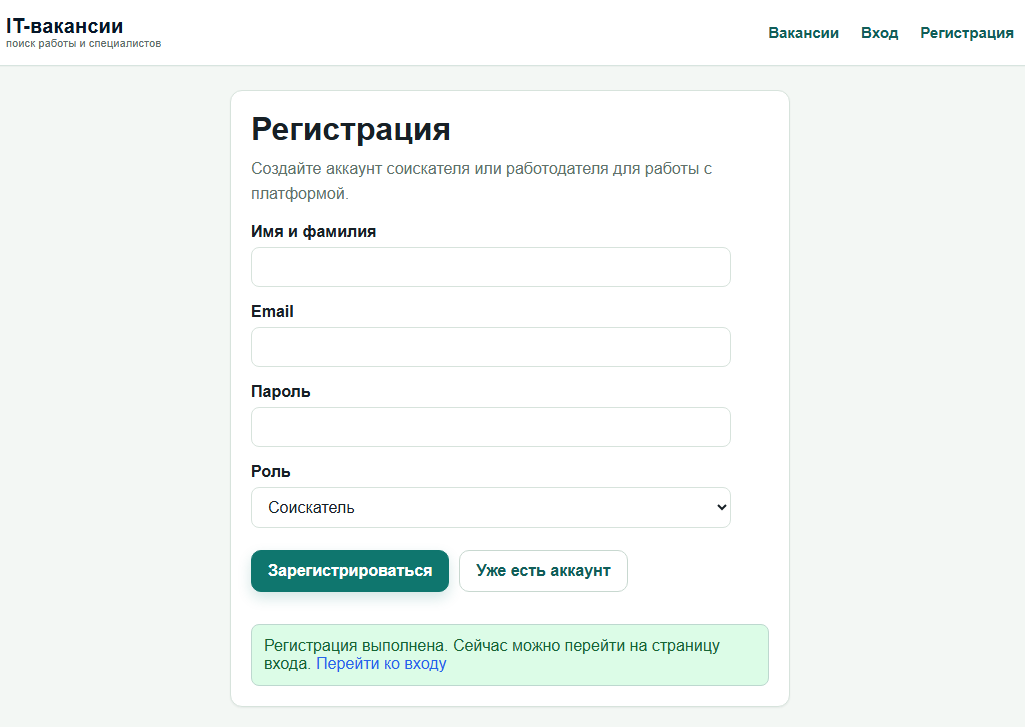
\includegraphics[width=1\linewidth]{tc01_registration.png}}
	\caption{Результат регистрации пользователя}
	\label{tc01:image}
\end{figure}

\subsubsection{TC-02. Вход пользователя в систему}

Цель тест-кейса: проверить корректность входа зарегистрированного пользователя в систему.

Предусловие: в системе существует зарегистрированная учётная запись пользователя, пользователь находится на странице входа.

Шаги выполнения тест-кейса:
\begin{enumerate}
	\item Открыть страницу входа.
	\item Ввести адрес электронной почты зарегистрированного пользователя.
	\item Ввести пароль пользователя.
	\item Нажать кнопку входа.
\end{enumerate}

Ожидаемый результат: система проверяет введённые учётные данные, выполняет вход пользователя и открывает доступ к функциям, соответствующим его роли.

Фактический результат: после ввода корректных учётных данных пользователь успешно входит в систему, сервер создаёт сеанс авторизации, а интерфейс открывает доступ к разделам, соответствующим роли пользователя. Тест-кейс пройден.

На рисунке \ref{tc02:image} представлен личный кабинет соискателя после успешного входа в систему.

\begin{figure}[H]
	\center{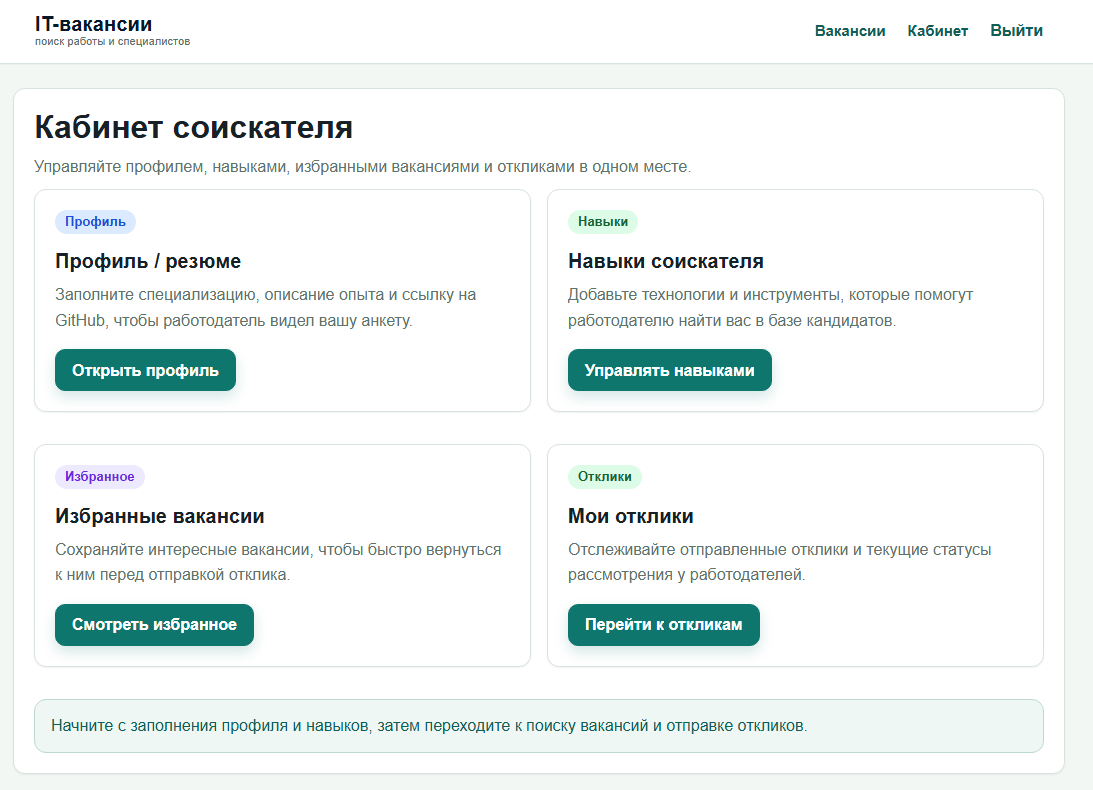
\includegraphics[width=1\linewidth]{tc02_login.png}}
	\caption{Личный кабинет соискателя после входа в систему}
	\label{tc02:image}
\end{figure}

\subsubsection{TC-03. Создание и редактирование профиля соискателя}

Цель тест-кейса: проверить возможность создания и редактирования профиля соискателя.

Предусловие: пользователь зарегистрирован в системе с ролью соискателя и выполнил вход в систему.

Шаги выполнения тест-кейса:
\begin{enumerate}
	\item Открыть личный кабинет соискателя.
	\item Перейти на страницу профиля.
	\item Заполнить сведения о специализации, описании опыта и ссылке на GitHub.
	\item Сохранить профиль.
	\item Изменить одно или несколько полей профиля.
	\item Повторно сохранить изменения.
\end{enumerate}

Ожидаемый результат: система создаёт профиль соискателя, сохраняет введённые данные и позволяет владельцу профиля редактировать их.

Фактический результат: профиль соискателя был создан, сведения о специализации, описании опыта и ссылке на GitHub сохранились в системе. После редактирования обновлённые данные отобразились на странице профиля. Тест-кейс пройден.

На рисунке \ref{tc03:image} представлен результат заполнения профиля соискателя.

\begin{figure}[H]
	\center{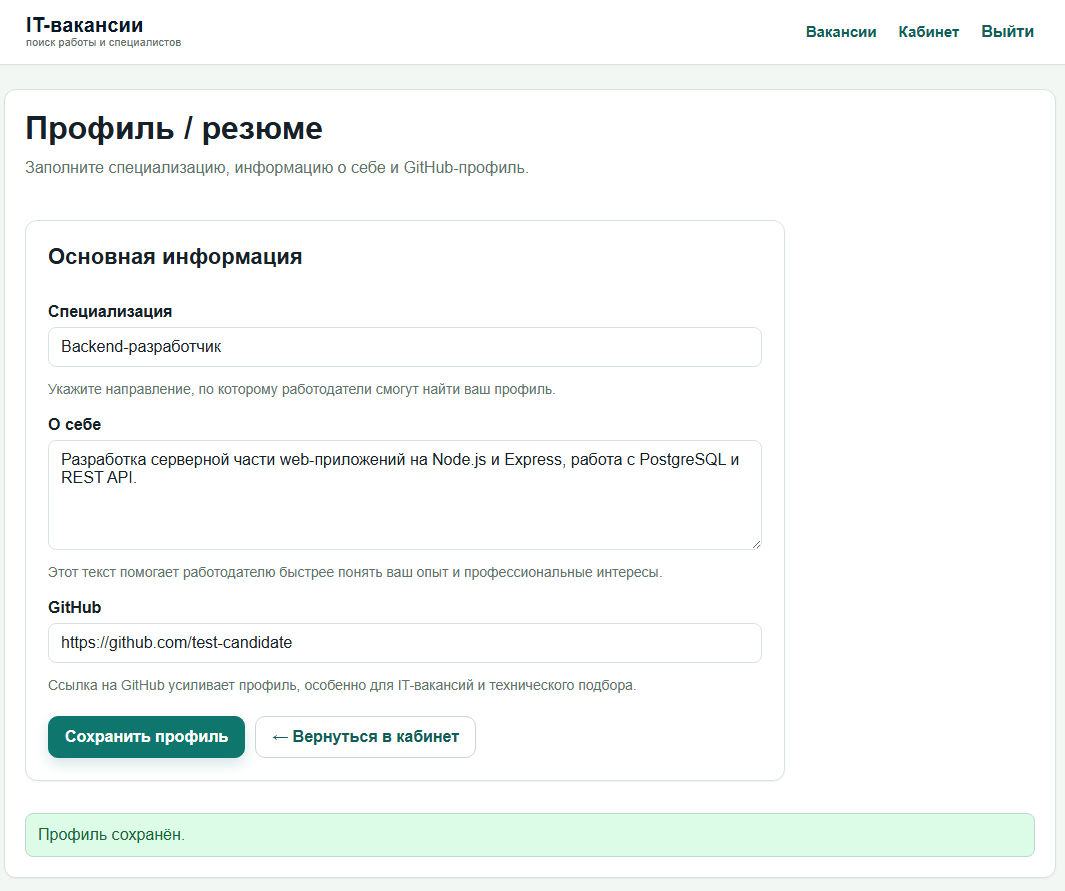
\includegraphics[width=1\linewidth]{tc03_candidate_profile.png}}
	\caption{Заполненный профиль соискателя}
	\label{tc03:image}
\end{figure}

\subsubsection{TC-04. Поиск и фильтрация вакансий}

Цель тест-кейса: проверить корректность поиска и фильтрации опубликованных вакансий.

Предусловие: в системе существуют опубликованные вакансии, пользователь находится на странице списка вакансий.

Шаги выполнения тест-кейса:
\begin{enumerate}
	\item Открыть страницу со списком вакансий.
	\item Ввести поисковый запрос в поле поиска.
	\item Указать параметры фильтрации, например специализацию, формат работы или тип занятости.
	\item Применить фильтр.
	\item Открыть одну из найденных вакансий.
\end{enumerate}

Ожидаемый результат: система отображает список вакансий, соответствующих заданным параметрам поиска и фильтрации, а также позволяет открыть карточку выбранной вакансии.

Фактический результат: после применения параметров поиска и фильтрации список вакансий обновился, в нём остались предложения, соответствующие заданным условиям. Карточка выбранной вакансии открылась и отобразила подробные сведения о вакансии. Тест-кейс пройден.

На рисунке \ref{tc04:image} представлен результат поиска и фильтрации вакансий.

\begin{figure}[H]
	\center{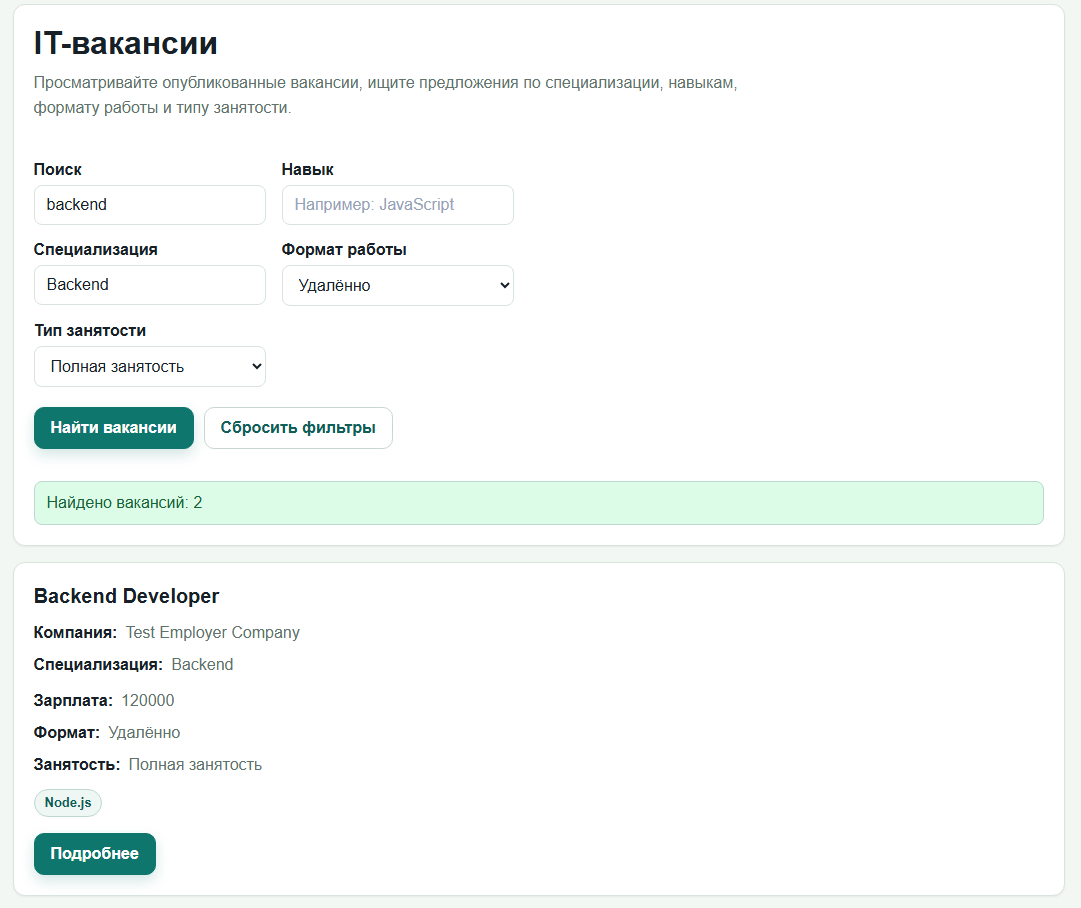
\includegraphics[width=1\linewidth]{tc04_vacancy_filter.png}}
	\caption{Результат поиска и фильтрации вакансий}
	\label{tc04:image}
\end{figure}

\subsubsection{TC-05. Отклик на вакансию}

Цель тест-кейса: проверить возможность отправки отклика соискателем на опубликованную вакансию.

Предусловие: пользователь зарегистрирован с ролью соискателя, выполнил вход в систему, имеет созданный профиль соискателя, в системе существует опубликованная вакансия.

Шаги выполнения тест-кейса:
\begin{enumerate}
	\item Открыть страницу со списком опубликованных вакансий.
	\item Выбрать подходящую вакансию.
	\item Открыть карточку выбранной вакансии.
	\item Нажать кнопку отправки отклика.
	\item Проверить появление отклика в списке собственных откликов соискателя.
\end{enumerate}

Ожидаемый результат: система создаёт отклик на выбранную вакансию, связывает его с профилем соискателя и отображает отклик в списке заявок пользователя.

Фактический результат: после нажатия кнопки отправки отклика в системе была создана запись отклика, связанная с выбранной вакансией и профилем текущего соискателя. Отклик отобразился в списке собственных откликов пользователя и получил начальный статус \texttt{new}. Тест-кейс пройден.

На рисунке \ref{tc05:image} представлен результат отправки отклика на вакансию.

\begin{figure}[H]
	\center{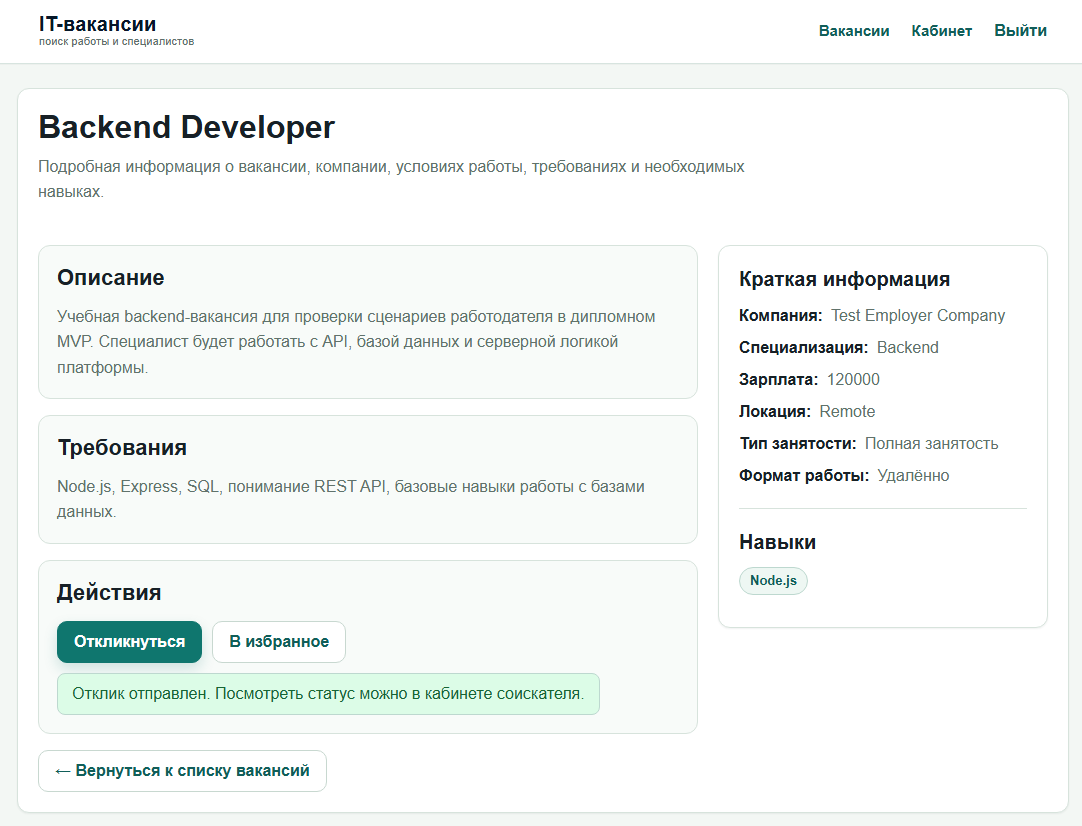
\includegraphics[width=1\linewidth]{tc05_application.png}}
	\caption{Результат отправки отклика на вакансию}
	\label{tc05:image}
\end{figure}

\subsubsection{TC-06. Добавление вакансии в избранное}

Цель тест-кейса: проверить возможность добавления опубликованной вакансии в список избранных вакансий соискателя.

Предусловие: пользователь зарегистрирован с ролью соискателя, выполнил вход в систему, в системе существует опубликованная вакансия.

Шаги выполнения тест-кейса:
\begin{enumerate}
	\item Открыть страницу со списком опубликованных вакансий.
	\item Выбрать интересующую вакансию.
	\item Нажать кнопку добавления вакансии в избранное.
	\item Перейти в раздел избранных вакансий.
	\item Проверить наличие выбранной вакансии в списке избранного.
\end{enumerate}

Ожидаемый результат: система добавляет выбранную вакансию в список избранных вакансий текущего пользователя и отображает её в соответствующем разделе.

Фактический результат: выбранная опубликованная вакансия была добавлена в список избранных вакансий текущего соискателя. При переходе в раздел избранного вакансия отобразилась вместе с основными сведениями о предложении и компании. Тест-кейс пройден.

На рисунке \ref{tc06:image} представлен результат добавления вакансии в избранное.

\begin{figure}[H]
	\center{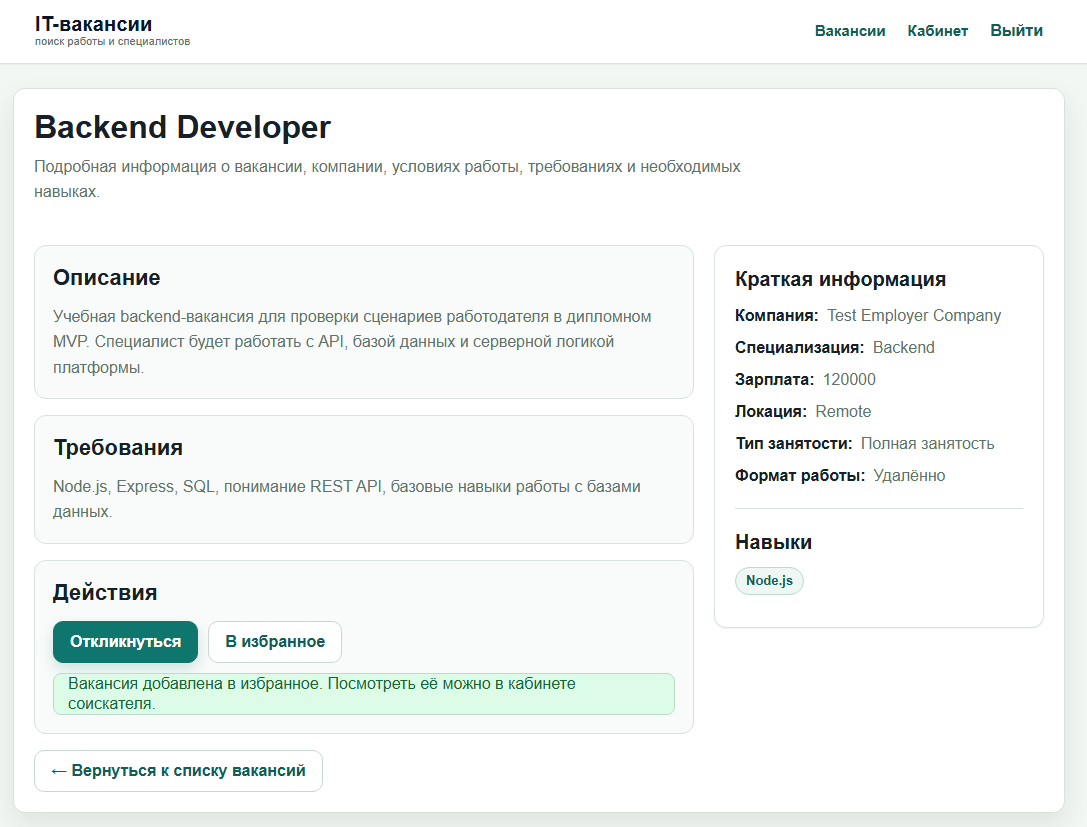
\includegraphics[width=1\linewidth]{tc06_favorites.png}}
	\caption{Результат добавления вакансии в избранное}
	\label{tc06:image}
\end{figure}

\subsubsection{TC-07. Создание и редактирование компании}

Цель тест-кейса: проверить возможность создания и редактирования профиля компании работодателем.

Предусловие: пользователь зарегистрирован с ролью работодателя и выполнил вход в систему.

Шаги выполнения тест-кейса:
\begin{enumerate}
	\item Открыть личный кабинет работодателя.
	\item Перейти на страницу управления компанией.
	\item Заполнить название компании, описание и адрес сайта.
	\item Сохранить данные компании.
	\item Изменить одно или несколько полей компании.
	\item Повторно сохранить изменения.
\end{enumerate}

Ожидаемый результат: система создаёт профиль компании, связывает его с текущим работодателем и позволяет владельцу компании редактировать её данные.

Фактический результат: профиль компании был создан и связан с учётной записью текущего работодателя. После редактирования изменённые сведения о названии, описании или сайте компании сохранились и отобразились в интерфейсе работодателя. Тест-кейс пройден.

\subsubsection{TC-08. Создание и публикация вакансии}

Цель тест-кейса: проверить возможность создания вакансии работодателем и её последующей публикации.

Предусловие: пользователь зарегистрирован с ролью работодателя, выполнил вход в систему и имеет созданный профиль компании.

Шаги выполнения тест-кейса:
\begin{enumerate}
	\item Открыть личный кабинет работодателя.
	\item Перейти на страницу управления вакансиями.
	\item Создать новую вакансию, заполнив название, специализацию, описание, требования, тип занятости и формат работы.
	\item Сохранить вакансию.
	\item Выполнить публикацию созданной вакансии.
	\item Перейти на страницу списка опубликованных вакансий.
	\item Проверить наличие опубликованной вакансии в общем списке.
\end{enumerate}

Ожидаемый результат: система создаёт вакансию, связывает её с компанией работодателя, переводит вакансию в опубликованный статус и отображает её в общем списке вакансий.

Фактический результат: вакансия была создана от имени компании текущего работодателя, после публикации получила статус опубликованной и стала доступна в общем списке вакансий для просмотра пользователями платформы. Тест-кейс пройден.

На рисунке \ref{tc08:image} представлен результат публикации вакансии работодателем.

\begin{figure}[H]
	\center{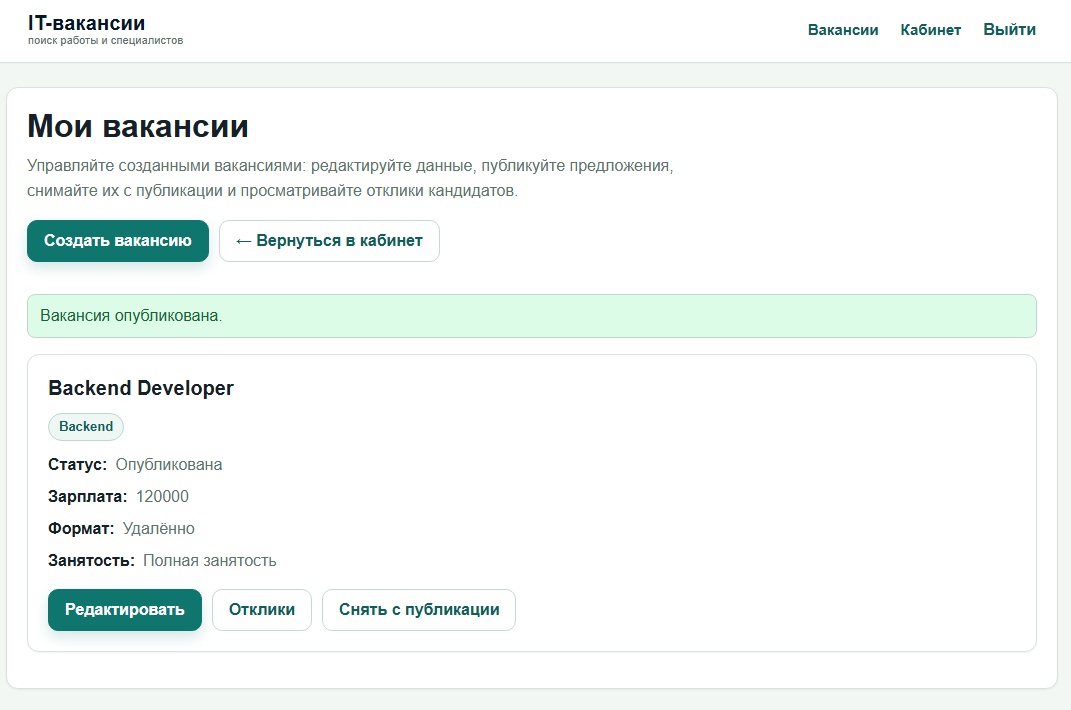
\includegraphics[width=1\linewidth]{tc08_publish_vacancy.png}}
	\caption{Результат публикации вакансии работодателем}
	\label{tc08:image}
\end{figure}

\subsubsection{TC-09. Просмотр откликов работодателем}

Цель тест-кейса: проверить возможность просмотра работодателем откликов, поступивших на принадлежащую ему вакансию.

Предусловие: пользователь зарегистрирован с ролью работодателя, выполнил вход в систему, имеет созданную компанию и опубликованную вакансию. В системе существует отклик соискателя на данную вакансию.

Шаги выполнения тест-кейса:
\begin{enumerate}
	\item Открыть личный кабинет работодателя.
	\item Перейти на страницу управления вакансиями.
	\item Выбрать опубликованную вакансию, на которую был отправлен отклик.
	\item Открыть список откликов по выбранной вакансии.
	\item Проверить отображение сведений о соискателе и статусе отклика.
\end{enumerate}

Ожидаемый результат: система отображает список откликов, связанных с выбранной вакансией работодателя, включая сведения о соискателях и текущие статусы откликов.

Фактический результат: после открытия списка откликов работодатель увидел заявки, связанные с выбранной вакансией. В интерфейсе отобразились сведения о соискателях, их профилях и текущих статусах откликов. Тест-кейс пройден.

На рисунке \ref{tc09:image} представлен список откликов, поступивших на вакансию работодателя.

\begin{figure}[H]
	\center{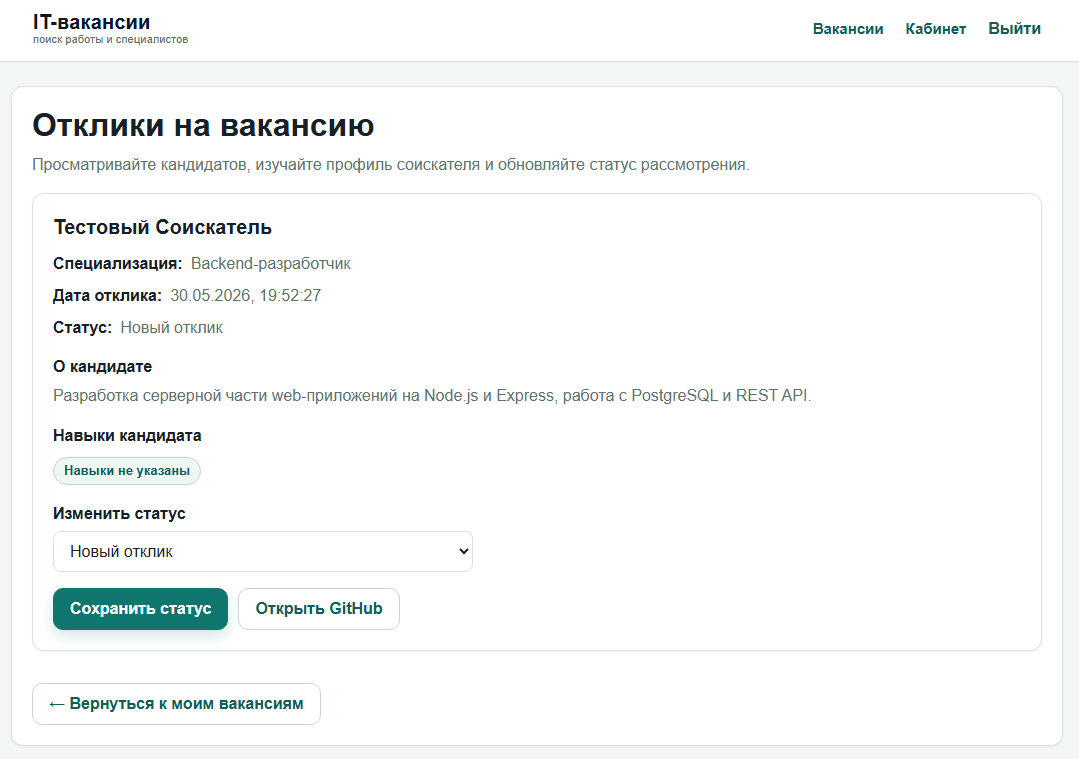
\includegraphics[width=1\linewidth]{tc09_employer_applications.png}}
	\caption{Список откликов на вакансию работодателя}
	\label{tc09:image}
\end{figure}

\subsubsection{TC-10. Изменение статуса отклика}

Цель тест-кейса: проверить возможность изменения работодателем статуса отклика на принадлежащую ему вакансию.

Предусловие: пользователь зарегистрирован с ролью работодателя, выполнил вход в систему, имеет опубликованную вакансию и полученный отклик от соискателя.

Шаги выполнения тест-кейса:
\begin{enumerate}
	\item Открыть личный кабинет работодателя.
	\item Перейти к списку откликов на выбранную вакансию.
	\item Выбрать отклик соискателя.
	\item Изменить статус отклика, например на \texttt{in\_review}, \texttt{accepted} или \texttt{rejected}.
	\item Сохранить изменение статуса.
	\item Проверить, что новый статус отображается в интерфейсе работодателя и в списке откликов соискателя.
\end{enumerate}

Ожидаемый результат: система изменяет статус выбранного отклика и сохраняет новое значение в базе данных.

Фактический результат: выбранный отклик получил новый статус, изменение сохранилось в системе и отобразилось в интерфейсе работодателя. Обновлённый статус также стал доступен соискателю в списке его откликов. Тест-кейс пройден.

На рисунке \ref{tc10:image} представлен результат изменения статуса отклика работодателем.

\begin{figure}[H]
	\center{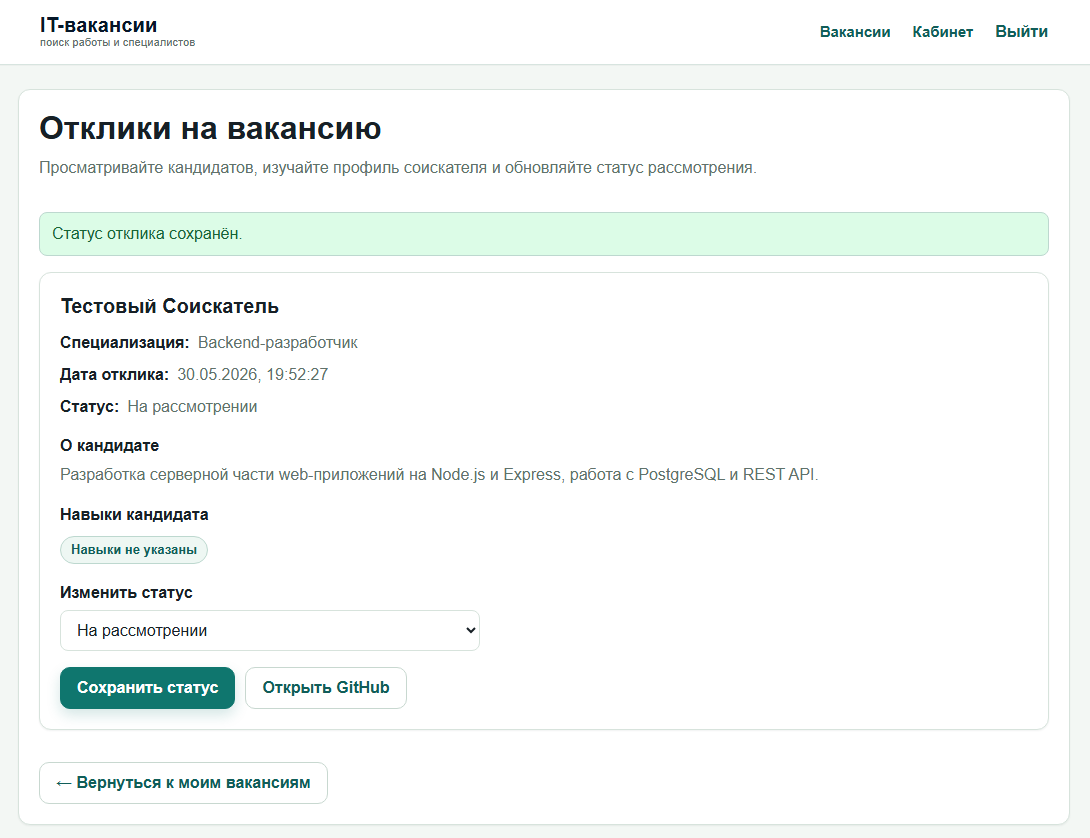
\includegraphics[width=1\linewidth]{tc10_application_status.png}}
	\caption{Результат изменения статуса отклика}
	\label{tc10:image}
\end{figure}

\subsubsection{TC-11. Поиск и фильтрация кандидатов}

Цель тест-кейса: проверить возможность поиска и фильтрации профилей соискателей работодателем.

Предусловие: пользователь зарегистрирован с ролью работодателя, выполнил вход в систему, в системе существуют профили соискателей с заполненной специализацией и навыками.

Шаги выполнения тест-кейса:
\begin{enumerate}
	\item Открыть личный кабинет работодателя.
	\item Перейти на страницу поиска кандидатов.
	\item Ввести значение специализации или выбрать навык для фильтрации.
	\item Применить параметры поиска.
	\item Открыть профиль одного из найденных соискателей.
\end{enumerate}

Ожидаемый результат: система отображает список профилей соискателей, соответствующих заданным параметрам поиска и фильтрации, а также позволяет открыть подробную информацию о выбранном кандидате.

Фактический результат: после применения параметров поиска список кандидатов обновился, и в нём отобразились профили соискателей, соответствующие выбранной специализации или навыку. Профиль выбранного кандидата открылся и отобразил профессиональные сведения соискателя. Тест-кейс пройден.

На рисунке \ref{tc11:image} представлен результат поиска и фильтрации кандидатов работодателем.

\begin{figure}[H]
	\center{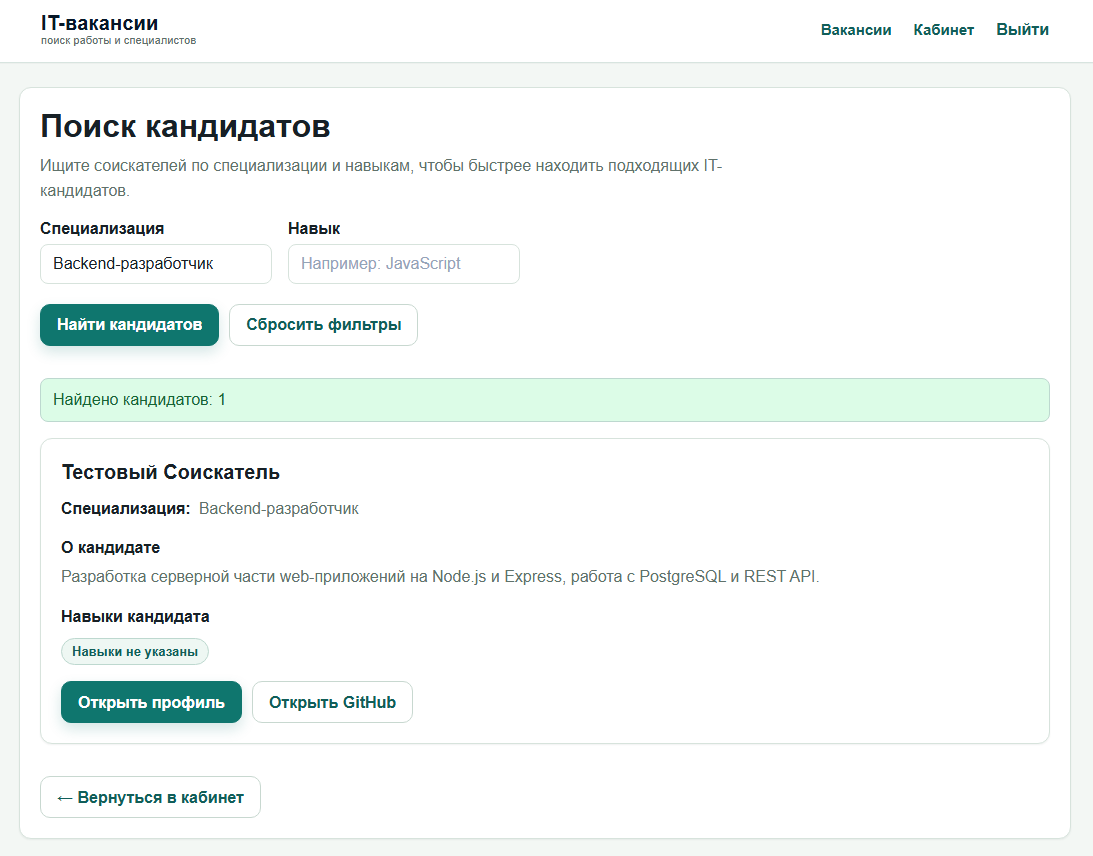
\includegraphics[width=1\linewidth]{tc11_candidate_search.png}}
	\caption{Результат поиска и фильтрации кандидатов}
	\label{tc11:image}
\end{figure}

\subsubsection{TC-12. Административное управление пользователями и вакансиями}

Цель тест-кейса: проверить возможность выполнения административных действий по управлению пользователями и вакансиями.

Предусловие: пользователь зарегистрирован с ролью администратора и выполнил вход в систему. В системе существуют зарегистрированные пользователи и созданные вакансии.

Шаги выполнения тест-кейса:
\begin{enumerate}
	\item Открыть личный кабинет администратора.
	\item Перейти на страницу управления пользователями.
	\item Проверить отображение списка пользователей.
	\item Выполнить блокировку выбранного пользователя.
	\item Перейти на страницу управления вакансиями.
	\item Проверить отображение списка вакансий.
	\item Выполнить удаление выбранной вакансии.
\end{enumerate}

Ожидаемый результат: система отображает списки пользователей и вакансий, позволяет администратору заблокировать пользователя и удалить выбранную вакансию.

Фактический результат: в административном интерфейсе отобразились списки пользователей и вакансий. После выполнения блокировки у выбранного пользователя был изменён признак доступа к системе, а выбранная вакансия была удалена из списка вакансий. Тест-кейс пройден.

На рисунке \ref{tc12:image} представлен интерфейс административного управления пользователями.

\begin{figure}[H]
	\center{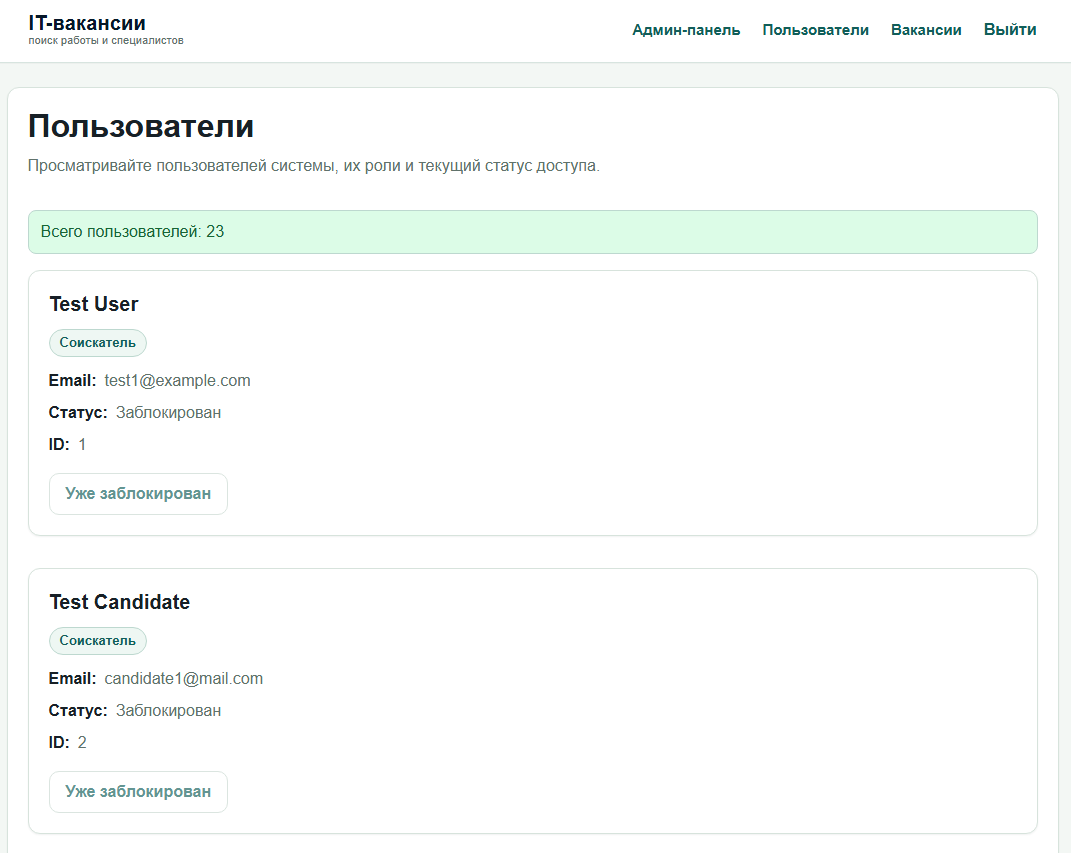
\includegraphics[width=1\linewidth]{tc12_admin_panel.png}}
	\caption{Интерфейс административного управления пользователями}
	\label{tc12:image}
\end{figure}

\subsubsection{TC-13. Проверка разграничения прав доступа}

Цель тест-кейса: проверить корректность ограничения доступа к функциям программной системы в зависимости от роли пользователя.

Предусловие: в системе существуют пользователи с ролями соискателя, работодателя и администратора.

Шаги выполнения тест-кейса:
\begin{enumerate}
	\item Открыть защищённую страницу без выполнения входа в систему.
	\item Проверить реакцию системы на попытку доступа без авторизации.
	\item Выполнить вход в систему под учётной записью соискателя.
	\item Попытаться открыть страницу управления компанией или вакансиями работодателя.
	\item Выполнить вход в систему под учётной записью работодателя.
	\item Попытаться открыть функции, предназначенные для соискателя, например управление избранными вакансиями.
	\item Выполнить вход в систему под обычной учётной записью и попытаться открыть административный раздел.
	\item Выполнить вход в систему под учётной записью администратора и проверить доступ к административным функциям.
\end{enumerate}

Ожидаемый результат: система запрещает доступ к защищённым страницам без авторизации, не позволяет пользователям выполнять действия, не соответствующие их роли, и предоставляет доступ к административным функциям только пользователю с ролью администратора.

Фактический результат: при попытке открыть защищённые страницы без авторизации система не предоставила доступ к закрытым функциям. Пользователи с ролями соискателя, работодателя и администратора получили доступ только к тем разделам, которые соответствуют их роли, а попытки обращения к недоступным функциям были заблокированы. Тест-кейс пройден.

На рисунке \ref{tc13:image} представлен результат попытки открытия защищённого раздела без авторизации.

\begin{figure}[H]
	\center{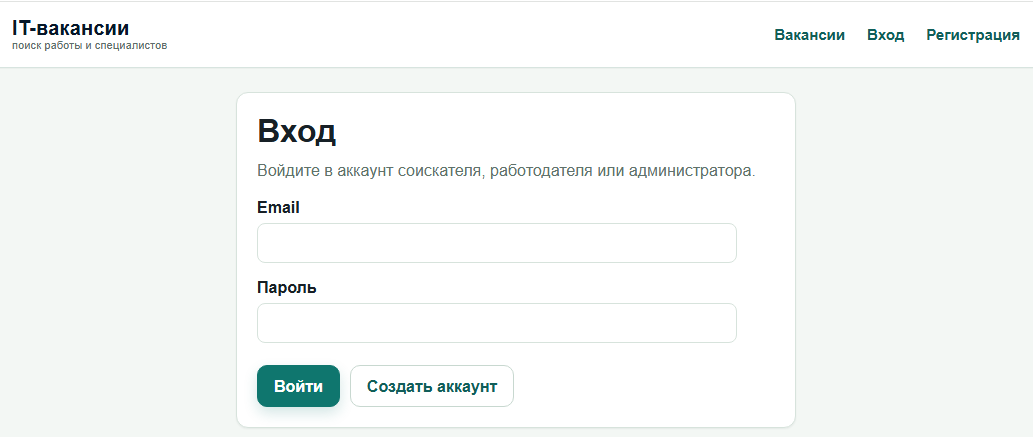
\includegraphics[width=1\linewidth]{tc13_access_control.png}}
	\caption{Результат ограничения доступа к защищённому разделу}
	\label{tc13:image}
\end{figure}

\subsubsection{Нефункциональное тестирование}

Помимо проверки основных пользовательских сценариев было выполнено нефункциональное тестирование программной системы. Оно было направлено на проверку корректности работы интерфейса, обработки ошибочных ситуаций, ограничения доступа и устойчивости системы к некорректным действиям пользователя.

В ходе нефункционального тестирования проверялась работа защищённых страниц. При попытке открытия личного кабинета без авторизации система не предоставляла доступ к закрытым функциям и перенаправляла пользователя к странице входа. Также проверялись действия пользователей с разными ролями. Соискатель не получал доступ к функциям работодателя и администратора, работодатель не получал доступ к административным функциям, а административные действия были доступны только пользователю с соответствующей ролью.

Отдельно проверялась обработка некорректных данных. При отправке форм с незаполненными обязательными полями система не выполняла операцию и отображала сообщение об ошибке. Такая проверка выполнялась для форм регистрации, входа, создания профиля соискателя, создания компании и создания вакансии.

Также проверялись ограничения повторных действий. Система не позволяла повторно отправить отклик на одну и ту же вакансию и повторно добавить одну и ту же вакансию в избранное. При выполнении таких действий пользователь получал сообщение об ошибке, а данные в системе не дублировались.

Проверка интерфейса показала, что основные страницы web-платформы корректно отображают данные, полученные от серверной части: списки вакансий, карточки вакансий, профили соискателей, сведения о компаниях, отклики, избранные вакансии и административные списки. При успешном выполнении операций пользователь получает соответствующее уведомление, а при ошибке отображается сообщение с причиной невозможности выполнения действия.

Таким образом, нефункциональное тестирование подтвердило корректную обработку ошибок, работу ограничений доступа, отсутствие дублирования данных при повторных действиях и корректное взаимодействие клиентской части с серверным API.

\subsubsection{Вывод по результатам тестирования}

По результатам системного тестирования было подтверждено, что основные функции разработанной web-платформы работают корректно. Проверка охватила основные пользовательские сценарии для гостя, соискателя, работодателя и администратора.

В ходе тестирования было установлено, что пользователь может зарегистрироваться и выполнить вход в систему, соискатель может создать и редактировать профиль, выполнять поиск вакансий, отправлять отклики и добавлять вакансии в избранное. Работодатель может создать профиль компании, создавать и публиковать вакансии, просматривать отклики соискателей, изменять их статусы и выполнять поиск кандидатов. Администратор может просматривать пользователей и вакансии, блокировать пользователей и удалять вакансии.

Также была проверена корректность разграничения прав доступа. Пользователи получают доступ только к тем функциям, которые соответствуют их роли. Попытки обращения к защищённым страницам без авторизации или к функциям другой роли блокируются системой.

Нефункциональное тестирование подтвердило корректную обработку ошибочных ситуаций, запрет повторных действий, таких как повторный отклик на одну вакансию или повторное добавление вакансии в избранное, а также корректное отображение сообщений об ошибках в пользовательском интерфейсе.

Таким образом, результаты тестирования подтверждают, что разработанная программная система реализует заявленные функциональные возможности и соответствует основным требованиям, сформулированным в техническом задании.
